\chapter{Evaluation}

% Requirements
% * Functional
% * Non-functional
%
% Algorithm
% * Gleichverteilt
% * Umfrage
%
% Implementation
% * scaling
% * ldap connections sind ne bitch
%
% Conclusion

\section{Fitness Score Algorithm}

\subsection{Uniform Distribution of Score Values}
The scores calculated by the algorithm should be distributed uniformly in the complete range of possible values, because this does not only generate the best search results, but also is an indicator for the algorithm's fairness.
To test this, one hundred persons have been fed into the system. Each test person has been assigned a random number of skills between zero and 17, with random skill and will levels each. A search for any skill will return a list of up to one hundred persons sorted by their fitness score. The search results for the skills \textit{Atomic Design}, \textit{Datenbanken}, \textit{Funkspots}, \textit{hybris}, \textit{Kommunikation}, \textit{MySQL}, \textit{Sktech} and \textit{Text} have been analyzed, because those have the highest number of results (33 each); all results can be found in table \ref{alldatatable}. Ideally, the scores in each result list decline linearily from one to zero. The ideal value for the $n$-th result value is:
\[
	v_{Ideal}(n) = 1 - \frac{n}{33}
\]

The distribution of the score values for every respective search is shown in figure \ref{fig:dist-raw}.
Figure \ref{fig:dist-avg} illustrates the average of all eight scores for each postion in the search result lists, the maximum value found at this position, and the respective minimum value.
It shows that the average score declines linearily, which means that the score values are distributed uniformly thorough the result lists. In figure \ref{fig:dist-raw}, every result function shows a variance from the ideal value; the average value in figure \ref{fig:dist-avg}, however, deviates signifitantly less from the ideal than any of the isolated data rows. This leads to the conclusion that the drift from the ideal that occurs when observering one single set of data for one specific search is based on the small amount of examined values (33 data points). The average fitness score shows an average error of approx. 6\% (see figure \ref{fig:dist-err}). The maximum error in the given set of data is 27\%.
This leads to the conclusion that the fitness score algorithm generates uniformly distributed score values with an acceptable error.\\
Interestingly, the maximum error seems to have a declining trend; the small amount of examined data does not provide a solid basis for assumptions about whether there is a systematic reason for this, and, if so, whether it could have a negative impact on the proper working of the system. Unfortunately, there is no authentic usage data yet, so that this question will remain unanswered and might be subject to further research.

\begin{figure}[H]
    \centering
    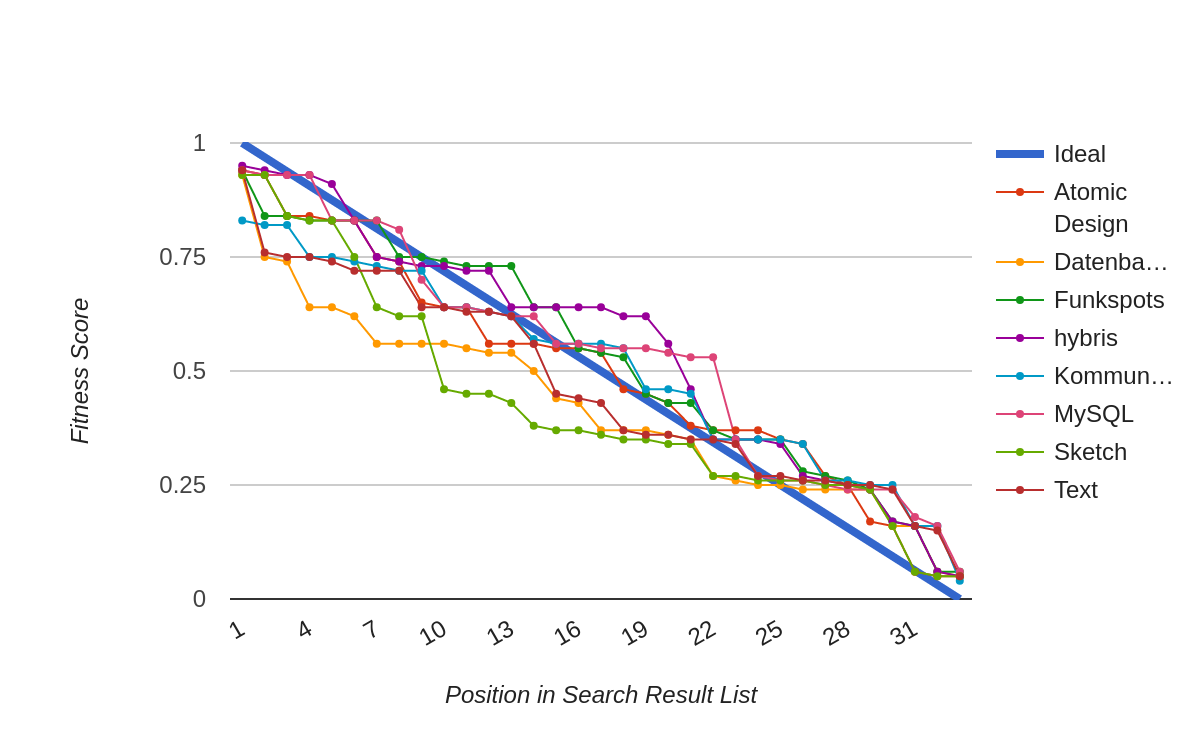
\includegraphics[width=\textwidth]{images/dist_raw.png}
    \caption[Raw Scores]{All search results and the ideal value.}
    \label{fig:dist-raw}
\end{figure}

\begin{figure}[H]
    \centering
    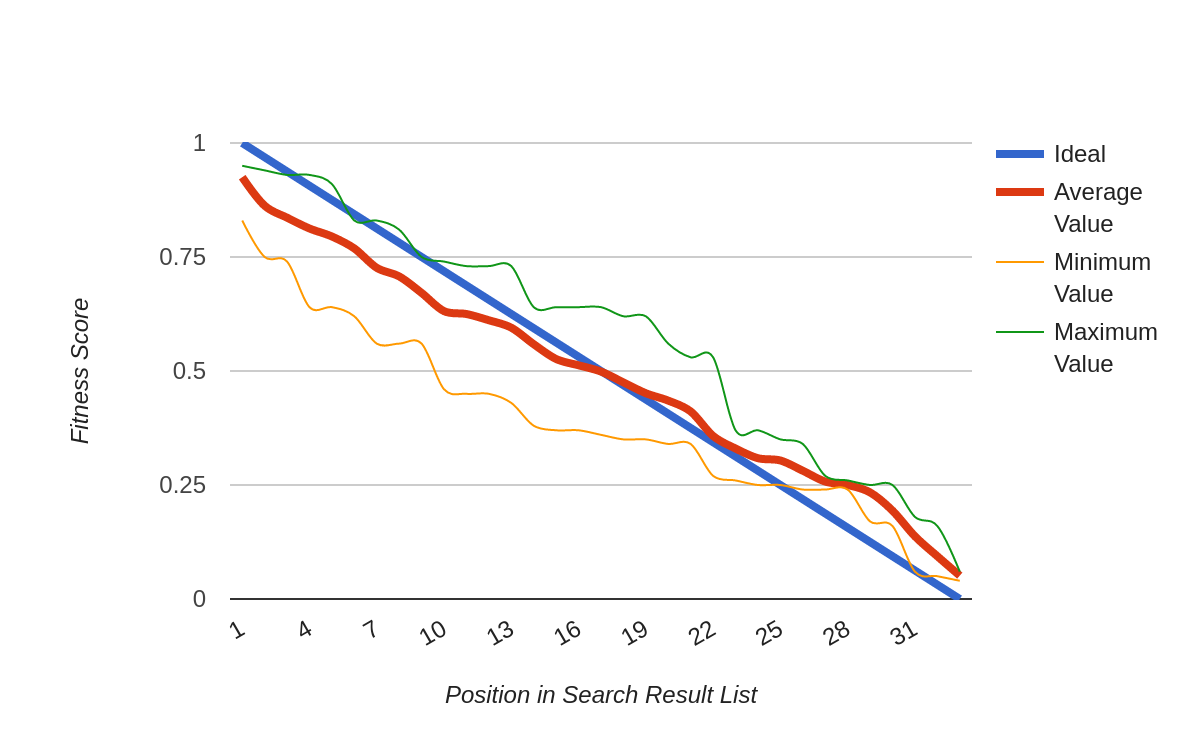
\includegraphics[width=\textwidth]{images/dist_avg.png}
    \caption[Average Scores]{Average, maximum and minimum score for earch position in the respective search result list.}
    \label{fig:dist-avg}
\end{figure}

\begin{figure}[H]
    \centering
    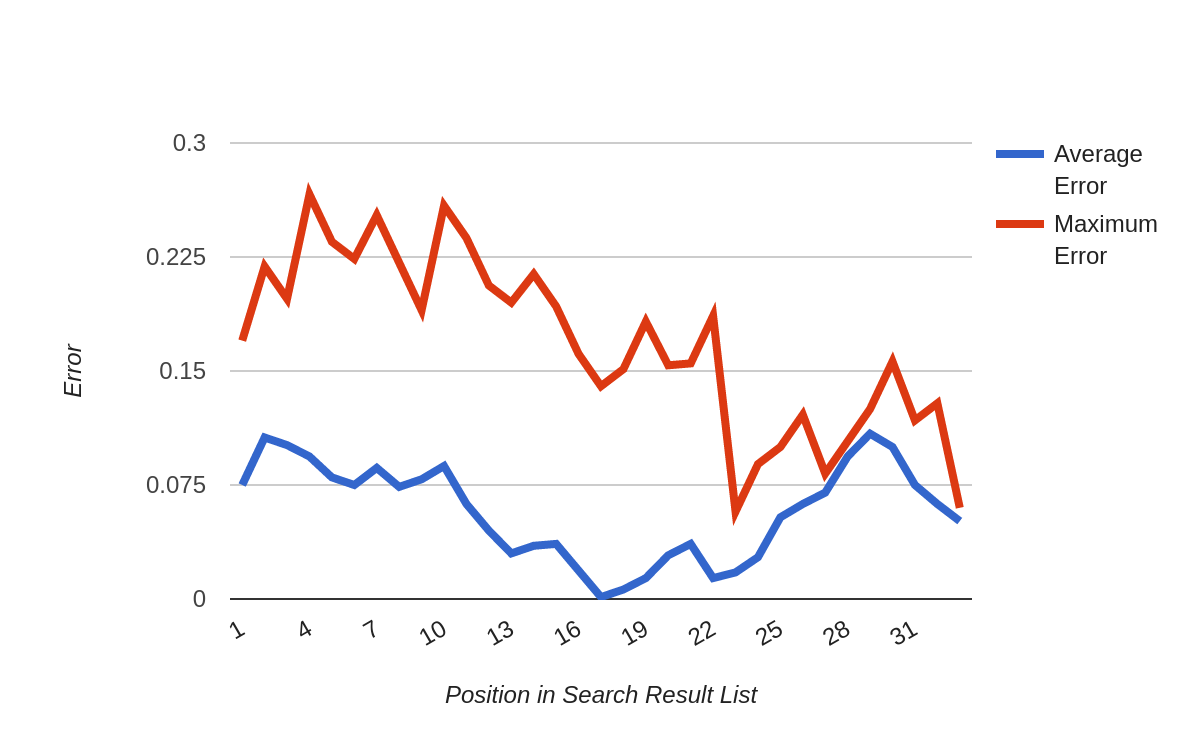
\includegraphics[width=\textwidth]{images/dist_error.png}
    \caption[Score Errors]{Average and maximum error (Difference between respective score value and the ideal value)}
    \label{fig:dist-err}
\end{figure}

\begin{table}[H]

\centering
\resizebox{\textwidth}{!}{
\rotatebox{-90}{
  \begin{tabular}{l||c|c|c|c|c|c|c|c|c||c|c|c||c|c}
	  No. & $v_{Ideal}$ & A.D. & DBs & Funk. & hybris & Kom. & MySQL & Sketch & Text & Avg. Val. & Min. Val. & Max. Val. & Avg. Err. & Max. Err.\\
	  \hline
	  1 & 1 & 0.94 & 0.93 & 0.94 & 0.95 & 0.83 & 0.94 & 0.93 & 0.94  &  0.925 & 0.83 & 0.95  &  0.075 & 0.17\\
 	 2 & 0.96875 & 0.93 & 0.75 & 0.84 & 0.94 & 0.82 & 0.93 & 0.93 & 0.76  &  0.8625 & 0.75 & 0.94  &  0.10625 & 0.21875\\
 	 3 & 0.9375 & 0.84 & 0.74 & 0.84 & 0.93 & 0.82 & 0.93 & 0.84 & 0.75  &  0.83625 & 0.74 & 0.93  &  0.10125 & 0.1975\\
 	 4 & 0.90625 & 0.84 & 0.64 & 0.83 & 0.93 & 0.75 & 0.93 & 0.83 & 0.75  &  0.8125 & 0.64 & 0.93  &  0.09375 & 0.26625\\
 	 5 & 0.875 & 0.83 & 0.64 & 0.83 & 0.91 & 0.75 & 0.83 & 0.83 & 0.74  &  0.795 & 0.64 & 0.91  &  0.08 & 0.235\\
 	 6 & 0.84375 & 0.83 & 0.62 & 0.83 & 0.83 & 0.74 & 0.83 & 0.75 & 0.72  &  0.76875 & 0.62 & 0.83  &  0.075 & 0.22375\\
 	 7 & 0.8125 & 0.75 & 0.56 & 0.83 & 0.75 & 0.73 & 0.83 & 0.64 & 0.72  &  0.72625 & 0.56 & 0.83  &  0.08625 & 0.2525\\
 	 8 & 0.78125 & 0.74 & 0.56 & 0.75 & 0.74 & 0.72 & 0.81 & 0.62 & 0.72  &  0.7075 & 0.56 & 0.81  &  0.07375 & 0.22125\\
 	 9 & 0.75 & 0.65 & 0.56 & 0.75 & 0.73 & 0.72 & 0.7 & 0.62 & 0.64  &  0.67125 & 0.56 & 0.75  &  0.07875 & 0.19\\
 	 10 & 0.71875 & 0.64 & 0.56 & 0.74 & 0.73 & 0.64 & 0.64 & 0.46 & 0.64  &  0.63125 & 0.46 & 0.74  &  0.0875 & 0.25875\\
 	 11 & 0.6875 & 0.64 & 0.55 & 0.73 & 0.72 & 0.64 & 0.64 & 0.45 & 0.63  &  0.625 & 0.45 & 0.73  &  0.0625 & 0.2375\\
 	 12 & 0.65625 & 0.56 & 0.54 & 0.73 & 0.72 & 0.63 & 0.63 & 0.45 & 0.63  &  0.61125 & 0.45 & 0.73  &  0.045 & 0.20625\\
 	 13 & 0.625 & 0.56 & 0.54 & 0.73 & 0.64 & 0.62 & 0.62 & 0.43 & 0.62  &  0.595 & 0.43 & 0.73  &  0.03 & 0.195\\
 	 14 & 0.59375 & 0.56 & 0.5 & 0.64 & 0.64 & 0.57 & 0.62 & 0.38 & 0.56  &  0.55875 & 0.38 & 0.64  &  0.035 & 0.21375\\
 	 15 & 0.5625 & 0.55 & 0.44 & 0.64 & 0.64 & 0.56 & 0.56 & 0.37 & 0.45  &  0.52625 & 0.37 & 0.64  &  0.03625 & 0.1925\\
 	 16 & 0.53125 & 0.55 & 0.43 & 0.55 & 0.64 & 0.56 & 0.56 & 0.37 & 0.44  &  0.5125 & 0.37 & 0.64  &  0.01875 & 0.16125\\
 	 17 & 0.5 & 0.54 & 0.37 & 0.54 & 0.64 & 0.56 & 0.55 & 0.36 & 0.43  &  0.49875 & 0.36 & 0.64  &  0.00125 & 0.14\\
 	 18 & 0.46875 & 0.46 & 0.37 & 0.53 & 0.62 & 0.55 & 0.55 & 0.35 & 0.37  &  0.475 & 0.35 & 0.62  &  0.00625 & 0.15125\\
 	 19 & 0.4375 & 0.45 & 0.37 & 0.45 & 0.62 & 0.46 & 0.55 & 0.35 & 0.36  &  0.45125 & 0.35 & 0.62  &  0.01375 & 0.1825\\
 	 20 & 0.40625 & 0.43 & 0.36 & 0.43 & 0.56 & 0.46 & 0.54 & 0.34 & 0.36  &  0.435 & 0.34 & 0.56  &  0.02875 & 0.15375\\
 	 21 & 0.375 & 0.38 & 0.35 & 0.43 & 0.46 & 0.45 & 0.53 & 0.34 & 0.35  &  0.41125 & 0.34 & 0.53  &  0.03625 & 0.155\\
 	 22 & 0.34375 & 0.37 & 0.27 & 0.37 & 0.35 & 0.35 & 0.53 & 0.27 & 0.35  &  0.3575 & 0.27 & 0.53  &  0.01375 & 0.18625\\
 	 23 & 0.3125 & 0.37 & 0.26 & 0.35 & 0.35 & 0.35 & 0.35 & 0.27 & 0.34  &  0.33 & 0.26 & 0.37  &  0.0175 & 0.0575\\
 	 24 & 0.28125 & 0.37 & 0.25 & 0.35 & 0.35 & 0.35 & 0.27 & 0.26 & 0.27  &  0.30875 & 0.25 & 0.37  &  0.0275 & 0.08875\\
 	 25 & 0.25 & 0.35 & 0.25 & 0.35 & 0.34 & 0.35 & 0.26 & 0.26 & 0.27  &  0.30375 & 0.25 & 0.35  &  0.05375 & 0.1\\
 	 26 & 0.21875 & 0.34 & 0.24 & 0.28 & 0.27 & 0.34 & 0.26 & 0.26 & 0.26  &  0.28125 & 0.24 & 0.34  &  0.0625 & 0.12125\\
 	 27 & 0.1875 & 0.27 & 0.24 & 0.27 & 0.26 & 0.26 & 0.25 & 0.25 & 0.26  &  0.2575 & 0.24 & 0.27  &  0.07 & 0.0825\\
 	 28 & 0.15625 & 0.25 & 0.24 & 0.26 & 0.25 & 0.26 & 0.24 & 0.25 & 0.25  &  0.25 & 0.24 & 0.26  &  0.09375 & 0.10375\\
 	 29 & 0.125 & 0.17 & 0.24 & 0.24 & 0.24 & 0.25 & 0.24 & 0.24 & 0.25  &  0.23375 & 0.17 & 0.25  &  0.10875 & 0.125\\
 	 30 & 0.09375 & 0.16 & 0.16 & 0.17 & 0.17 & 0.25 & 0.24 & 0.16 & 0.24  &  0.19375 & 0.16 & 0.25  &  0.1 & 0.15625\\
 	 31 & 0.0625 & 0.06 & 0.16 & 0.16 & 0.16 & 0.16 & 0.18 & 0.06 & 0.16  &  0.1375 & 0.06 & 0.18  &  0.075 & 0.1175\\
 	 32 & 0.03125 & 0.05 & 0.06 & 0.06 & 0.06 & 0.16 & 0.16 & 0.05 & 0.15  &  0.09375 & 0.05 & 0.16  &  0.0625 & 0.12875\\
 	 33 & 0 & 0.05 & 0.05 & 0.06 & 0.05 & 0.04 & 0.06 & 0.05 & 0.05  &  0.05125 & 0.04 & 0.06  &  0.05125 & 0.06\\
  \end{tabular}
}}
\caption[Fitness Score Test Distribution (Raw)]{Fitness score values that have been selected for this test.}
\label{alldatatable}
\end{table}

\newpage

\section{Implementation}
\subsection{Scalability}
A software system has to be able to scale according to the number of its users in order to be future-proof, as the current trend to dynamically scalable cloud solutions and server-less web architecture approaches highlights. There are two concepts or preparing an application for an higher workload: vertical scaling and horizontal scaling. Vertical scaling is done by providing more resources, e.g. Memory and CPU power, to the machines running the applicaions. Horziontal scaling, however, means setting up more machines providing the same service, so that workload can be distributed between them \cite{hvscale}. In contrast to vertical scaling, horizontal scaling has vital advantages: the application will be more robust since the crashing of one machine can be compensated by others \cite{fedi}, the capacity of the system can, theoretically, be unlimited, and it is cheaper, because instances can be created dynamically if needed and then be destroyed in times of low workload, whereas the resources given to a machine that has been scaled vertically will remain unused.

\begin{figure}[!htp]
    \centering
    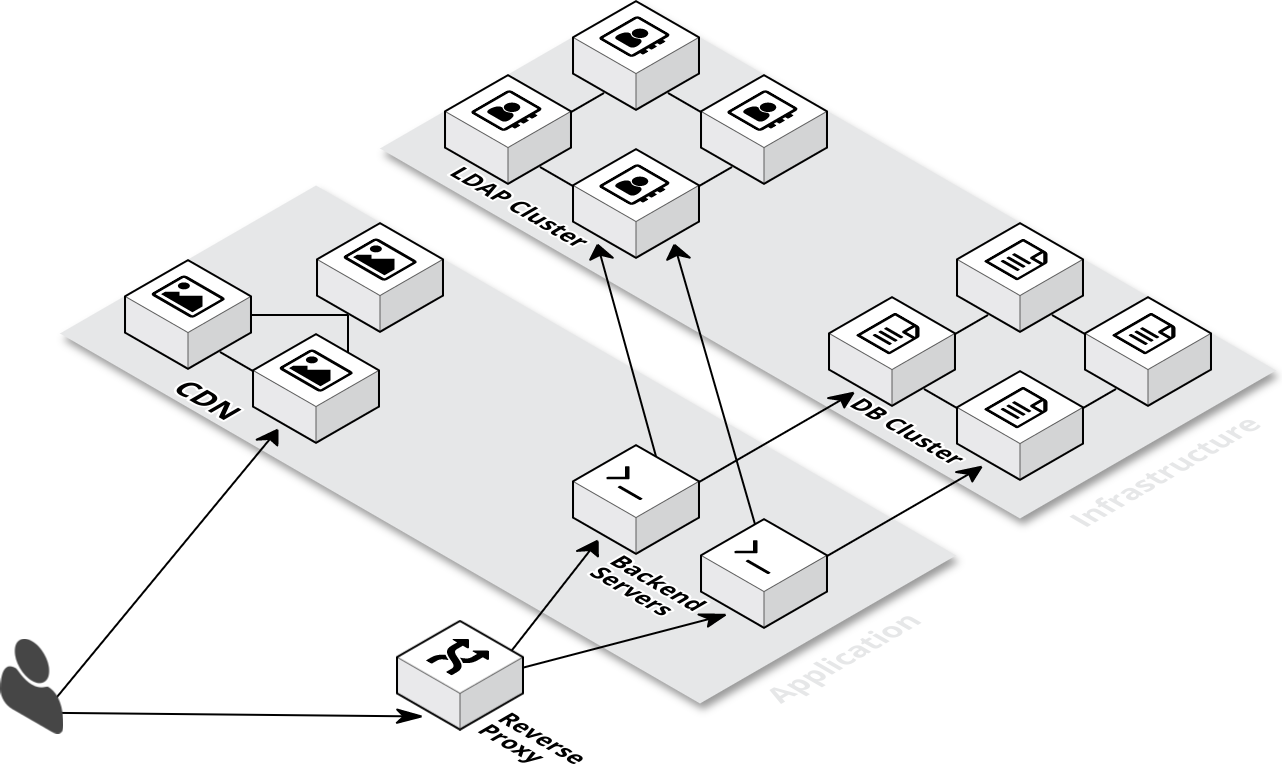
\includegraphics[width=0.75\textwidth]{images/system_architecture_scaled.png}
    \caption[System Architecture (scaled up)]{A possible approach to scale the system using multiple backend servers, a CDN, and multiple clustered database and ldap servers. Created with \textit{https://cloudcraft.co}.}
    \label{scaleup}
\end{figure}

\newpage
\subsubsection{MongoDB}
MongoDB is meant to be scaled horizontally and supports the adding of new instances to a running cluster of databases out-of-the-box \cite[p. 19]{MongoGuide}. So, new machines running the database as a cluster will be created, if needed. As shown in \ref{scaleup}, the backend servers can be connected to any of the database servers in order to request data. If the demanded document is not found on the instance the backend is connected to, MongoDB will handle the lookup in the cluster; to the application, the cluster is completely transparent and appear as if it was one machine.

\subsubsection{LDAP}
The LDAP servers\footnote{SinnerSchrader is running \textit{OpenLDAP} (http://www.openldap.org)} can also be run as a cluster in order to improve response times and prevent data loss by replicating the stored information \cite{ldapscale}. In fact, the LDAP is currently being provided by six servers that represent the service. As illustrated in \ref{scaleup}, the backend servers can connect to any of the LDAP servers; the data replication and synchronization is handled transparently.

\subsubsection{Static Content}
The static content files like HTML, CSS and JS files, that altogether represent the frontend, are
served by the reverse proxy web server. In the event of an increasing number of requests that cannot be handled by the single server, a \textit{Content Delivery Network} (CDN) could be deployed. A CDN is a network of webservers that provide static content and large files. The reverse proxy would redirect the URLs for those files, so that the users' browsers will connect directly to said network in order to retrieve the assets.

\subsubsection{Backend}
The backend application itself does not save any data on the machine it is running on, but connects a database server (see \ref{impl:be}). As a result, any number of backend instances can be set up. In contrast to the other services, the backend servers do not have to synchronize. In order to receive HTTP requests, the reverse proxy must be configured so that it redirects API calls to the backend servers. This is called \textit{load balancing} and is supported by many modern web servers such as \textit{nginx}, \textit{Apache} and \textit{Tomcat}.

\newpage

\subsection{Conclusion}
In theory, the application should be able to scale according to the number of its users. Practically, only the running of multiple backend and LDAP servers has been tested successfully. Running multiple database instances has not been tested; since MongoDB has been designed to be horizontally scalable and comes to use in various companies like
\textit{Github}\footnote{https://www.mongodb.com/presentations/mongosv-2012/mongodb-analytics-github},
\textit{eBay}\footnote{https://www.mongodb.com/presentations/mongodb-ebay}, and
\textit{Otto}\footnote{https://www.mongodb.com/industries/retail}, it can be assumed that this can be done successfully for this application, too.
Deploying a CDN that serves the static content has not been evaluated, as the implementation of the frontend was not part of this thesis, but has been worked on by \cite{strecker}.
